\documentclass[twocolumn]{revtex4-2}

\usepackage{amsmath,amssymb,amsthm}
\usepackage{graphicx}
\usepackage{booktabs}
\usepackage{xcolor}
\usepackage{hyperref}

\newtheorem{theorem}{Theorem}

\newcommand{\Nf}{N_f}
\newcommand{\Csq}{C^{2}}
\newcommand{\GB}{\mathcal{G}}
\newcommand{\Riem}{R_{\mu\nu\rho\sigma} R^{\mu\nu\rho\sigma}}
\newcommand{\Ric}{R_{\mu\nu} R^{\mu\nu}}
\newcommand{\Rsq}{R^{2}}
\newcommand{\Temerg}{T^{\mathrm{emerg}}}
\newcommand{\Tmatter}{T^{\mathrm{matter}}}
\newcommand{\aADW}{\alpha_{\mathrm{ADW}}}
\newcommand{\rhoADW}{\rho_{\mathrm{ADW}}}
\newcommand{\GN}{G_{N}}
\newcommand{\GNem}{G_{N}^{\mathrm{emerg}}}
\newcommand{\GNsak}{G_{N}^{\mathrm{Sakharov}}}

% Auto-generated by update_counts.py — 2026-04-24T19:44:03.140400
% Do not edit manually. Run: uv run python scripts/update_counts.py
\newcommand{\totaltheorems}{3993}
\newcommand{\substantivetheorems}{3882}
\newcommand{\placeholdertheorems}{111}
\newcommand{\axiomcount}{1}
\newcommand{\sorrycount}{0}
\newcommand{\sorrypercent}{0.0}
\newcommand{\leanmodules}{167}
\newcommand{\leandefinitions}{3297}
\newcommand{\pythonmodules}{68}
\newcommand{\testfiles}{59}
\newcommand{\totaltests}{2836}
\newcommand{\figurecount}{111}
\newcommand{\notebookcount}{54}
\newcommand{\papercount}{19}
\newcommand{\aristotleproved}{322}
\newcommand{\aristotleruns}{44}
% --- Paper 18 / Phase 5t per-section counts (FermiHubbardDimer.lean) ---
\newcommand{\fhdTotal}{143}
\newcommand{\fhdWaveTwo}{13}
\newcommand{\fhdWaveThree}{6}
\newcommand{\fhdWaveFour}{22}
\newcommand{\fhdWaveFive}{22}
\newcommand{\fhdWaveSixABC}{38}
\newcommand{\fhdWaveSixExtra}{15}
\newcommand{\fhdWaveSeven}{19}
\newcommand{\fhdWaveEight}{8}

% \nonlinearEFEThms and \nonlinearEFETests are auto-generated by
% scripts/update_counts.py from the canonical Lean source +
% pytest count and live in docs/counts.tex.

\begin{document}

\title{Variational nonlinear Einstein field equations from the ADW
  emergent-gravity programme: a Lean-formalized trace-level Decision Gate}

\author{John G. Roehm}
\affiliation{Independent Researcher; \texttt{NetRxn137@gmail.com}}

\date{\today}

\begin{abstract}
We formalize, in the Lean~4 proof assistant, the variational
trace-level Einstein field equations of the ADW emergent-gravity
programme through order $a_{4}$ of the Seeley--DeWitt heat-kernel
expansion. Variation of the effective action with respect to the
tetrad $e^{a}_{\mu}$ produces, at the trace level, a non-trivial
balance condition between the emergent stress-energy
$\Temerg = \aADW \cdot \rhoADW$, the bare-matter source $\Tmatter =
\rhoADW$, and the higher-curvature correction $\mathcal{A}_{4}$
inherited from Wave~2~\cite{HigherCurvature2026}. The substantive
correctness-push is a \emph{Decision-Gate-style biconditional}: under
positive Newton constant and non-zero matter source, the trace-level
EFE residual vanishes iff the ADW dimensionless coefficient is at the
Sakharov--Adler calibration $\aADW = 1$~\cite{Sakharov1968,
LinearizedEFE2026}. This is the nonlinear analogue of Wave~1's
Decision Gate~E.2~\cite{Roehm2026Wave1}. The bundled tracked-Prop
$H_{\mathrm{NonlinearEFEHolds}}$ is dispatched by three substantive
cross-bridges --- one each to Wave~1 (heat-kernel $\GN$), Wave~2
(higher-curvature pulsar bound), and Wave~3 (path-(b) diff
invariance)~\cite{DiffInvariance2026}. We extend the framework to
PPN-style multi-channel observables (light deflection, perihelion
precession, ringdown frequency) under the ADW $\aADW$ rescaling,
deriving the project-specific cross-channel structural claim that the
perihelion deviation is exactly $2/3$ of the deflection
deviation~\cite{Will2018, BertiCardosoStarinets2009}. The
\texttt{NonlinearEFE.lean} module ships \nonlinearEFEThms{}
substantive theorems, zero \texttt{sorry}, and zero new axioms; the
Python mirror in \texttt{src/nonlinear\_efe/} backs them with
\nonlinearEFETests{} cross-checks.
\end{abstract}

\maketitle

\section{Introduction}
\label{sec:intro}

In the ADW emergent-gravity programme, the gravitational sector
emerges from the one-loop fermion determinant of an underlying
$8$-fermion theory, expressed via a Seeley--DeWitt heat-kernel
expansion of $\det(\gamma^{a} \hat{E}^{a}_{\mu} D^{\mu})$. Phase~6e
Waves~1--3 formalised
\begin{enumerate}
\item the Christensen--Duff Dirac $a_{0}, a_{2}, a_{4}$
  coefficients in $4$D vacuum~\cite{Roehm2026Wave1,
  ChristensenDuff1979, Vassilevich2003};
\item the Stelle higher-curvature basis change at order
  $a_{4}$~\cite{HigherCurvature2026, Stelle1977};
\item the path-(b) diffeomorphism invariance of the resulting
  effective Lagrangian, with Decision Gate~E.3 returning
  PASS through order $a_{4}$~\cite{DiffInvariance2026, Wald1984}.
\end{enumerate}

The present paper takes the next step: variation of the resulting
effective action with respect to the tetrad to obtain the nonlinear
EFE itself.

The full tensor variational EFE
$\delta S/\delta e^{a}_{\mu} = 0$ produces, schematically,
\begin{equation}
  G_{\mu\nu} + \alpha_{\mathrm{HC}} \cdot \mathcal{A}_{4,\mu\nu}
    = 8\pi \GN \cdot \Temerg_{\mu\nu},
  \label{eq:full_tensor_efe}
\end{equation}
where $\mathcal{A}_{4,\mu\nu}$ is the variational $a_{4}$ correction
inheriting Wave~2's $(\alpha, \beta, \gamma)$ coefficients, and
$\Temerg_{\mu\nu}$ is the ADW-substrate-sourced emergent
stress-energy. Manifold-level formalization of this tensor equation
requires the Lorentzian differential-geometric infrastructure of
Phase~6f, which is not yet available. We therefore work at the
\emph{trace level}: scalar contraction of
Eq.~(\ref{eq:full_tensor_efe}) against $g^{\mu\nu}$ yields a
single-equation residual
\begin{equation}
  \mathcal{R}_{\mathrm{EFE}}(\GN, \rhoADW, \aADW)
    \equiv 8\pi \GN \cdot \rhoADW \cdot (\aADW - 1),
  \label{eq:residual_def}
\end{equation}
whose vanishing condition is precisely the Decision-Gate-style
biconditional this paper formalises in Lean. The trace-level
restriction preserves the load-bearing physics --- Newton-constant
calibration, emergent-vs-matter source comparison, observable PPN
deviations --- without requiring index machinery deferred to
Phase~6f.

\paragraph*{Scope lock.}
\textsc{In scope} for this paper:
\begin{enumerate}
\item Trace-level EFE residual under the ADW $\aADW$
  rescaling (\S~\ref{sec:residual});
\item Decision-Gate-style biconditional witnessing exact calibration
  ($\aADW = 1$) consistency (\S~\ref{sec:residual});
\item Linear deviation channel
  $\Temerg - \Tmatter = (\aADW - 1) \rhoADW$ (\S~\ref{sec:source});
\item PPN-style observable predictions (deflection, perihelion
  precession, ringdown frequency) under $\GN \to \aADW \GNsak$
  (\S~\ref{sec:observable});
\item Substantive cross-bridges to Waves~1, 2, 3
  (\S~\ref{sec:cross_bridges});
\item Bundled tracked-Prop
  $H_{\mathrm{NonlinearEFEHolds}}$ at the calibration value
  (\S~\ref{sec:bundle}).
\end{enumerate}
\textsc{Out of scope}: full tensor EFE on a manifold (deferred to
Phase~6f Lorentzian infrastructure); microscopic cosmological constant
$\Lambda^{\mathrm{emerg}}(\Lambda_{\mathrm{UV}}, \Nf, G_{c})$
(deferred to Wave~5); torsion-sourced extensions (deferred to Wave~6
Einstein--Cartan); two-loop quantum corrections (out of scope per
strategy doc \S15).

\section{Trace-level stress-energy under the ADW rescaling}
\label{sec:source}

The ADW substrate sources gravity through the one-loop fermion
determinant; at the linearized post-Newtonian level, this rescales
the emergent Newton constant by the dimensionless coefficient $\aADW$
(Phase~6a.1, \cite{LinearizedEFE2026}):
\begin{equation}
  \GNem(\Lambda, \Nf, \aADW) = \aADW \cdot \GNsak(\Lambda, \Nf),
\end{equation}
where $\GNsak = 12\pi/(\Nf \Lambda^{2})$ is the Sakharov--Adler
one-loop induced-gravity Newton constant. The Wave~1 heat-kernel
calibration $\GN = G_{N,\mathrm{from\;a_{2}}}$ matches $\GNsak$
exactly when $\aADW = 1$~\cite{Roehm2026Wave1}.

\subsection{Emergent vs bare-matter trace}

We define
\begin{align}
  \Temerg &\equiv \aADW \cdot \rhoADW, \label{eq:T_emerg_def}\\
  \Tmatter &\equiv \rhoADW. \label{eq:T_matter_def}
\end{align}
The deviation channel
\begin{equation}
  \Temerg - \Tmatter = (\aADW - 1) \cdot \rhoADW
  \label{eq:deviation_channel}
\end{equation}
is the load-bearing observable signature of the ADW substrate's
calibration deviation: it vanishes at $\aADW = 1$ and grows linearly
with $\aADW - 1$ otherwise. The biconditional in Lean,
\begin{equation}
  \rhoADW \neq 0 \;\Longrightarrow\;
   \big(\Temerg = \Tmatter \iff \aADW = 1\big),
\end{equation}
is the substantive content of theorem
\texttt{emergentStressEnergyTrace\_eq\_matter\_iff\_alpha\_unity}; the
linear-response form of Eq.~(\ref{eq:deviation_channel}) is
\texttt{emergentStressEnergyTrace\_minus\_matter\_eq}.

\section{Trace-level EFE residual and the Decision Gate biconditional}
\label{sec:residual}

\subsection{Residual definition}

The trace contraction of Eq.~(\ref{eq:full_tensor_efe}), with the
Sakharov--Adler-baseline Einstein + matter trace absorbed into the
calibrated configuration, gives a residual
\begin{equation}
  \mathcal{R}_{\mathrm{EFE}}(\GN, \rhoADW, \aADW)
    = 8\pi \GN \cdot \rhoADW \cdot (\aADW - 1),
  \label{eq:residual}
\end{equation}
which by construction \emph{vanishes identically at the calibration
$\aADW = 1$ for all $(\GN, \rhoADW)$}
(\texttt{efeResidualTrace\_at\_alpha\_one}).

\subsection{Decision-Gate-style biconditional}

The substantive Wave~4 result is the converse: under positive Newton
constant and non-zero matter source, $\mathcal{R}_{\mathrm{EFE}}$
vanishes \emph{only at} $\aADW = 1$.
\begin{theorem}[Wave~4 correctness-push]\label{thm:decision_gate}
For all $\GN, \rhoADW, \aADW \in \mathbb{R}$ with $\GN > 0$ and
$\rhoADW \neq 0$,
\begin{equation*}
  \mathcal{R}_{\mathrm{EFE}}(\GN, \rhoADW, \aADW) = 0
    \iff \aADW = 1.
\end{equation*}
\end{theorem}
\noindent The Lean proof of the biconditional
(\texttt{efeResidualTrace\_eq\_zero\_iff\_alpha\_unity}) reduces the
forward direction to $\rhoADW \cdot (\aADW - 1) = 0$ via $8\pi \GN
\neq 0$, then resolves $\aADW - 1 = 0$ using $\rhoADW \neq 0$. The
reverse direction is the calibration consistency
$\mathcal{R}_{\mathrm{EFE}}(\cdot, \cdot, 1) = 0$.

This is the nonlinear analogue of Wave~1's Decision Gate~E.2
biconditional
\texttt{a2\_matches\_GNemerg\_iff\_alpha\_ADW\_unity}~\cite{Roehm2026Wave1};
together they pin the Sakharov--Adler calibration as the unique
algebraic locus where both the linearized $a_{2}$ Einstein--Hilbert
prefactor and the nonlinear-EFE trace simultaneously close.

\subsection{Substantive cross-bridge to Wave~1 + Phase~6a.1}

At the Dirac+Sakharov calibration, the heat-kernel-derived Newton
constant equals the ADW emergent Newton constant at $\aADW = 1$, and
the EFE residual vanishes:
\begin{equation*}
  \mathcal{R}_{\mathrm{EFE}}(\GNem(\Lambda, \Nf, 1), \rhoADW, 1) = 0.
\end{equation*}
The Lean proof (\texttt{efeResidualTrace\_at\_dirac\_calibration\_vanishes})
invokes \texttt{LinearizedEFE.G\_N\_emerg\_at\_alpha\_one} (Phase~6a.1)
and \texttt{HeatKernelExpansion.G\_N\_from\_a2\_eq\_G\_N\_sakharov}
(Wave~1) by name, providing P6 cross-module bridge integrity per the
project's drift-protection convention.

\section{Multi-channel post-Newtonian observables}
\label{sec:observable}

The substantive content of Wave~4 at the observable level is a
\emph{multi-channel structural claim}: the ADW $\aADW$ rescaling
imprints the same dimensionless calibration parameter on three
canonical post-Newtonian observables, but with channel-dependent
functional forms.

\subsection{Light deflection}

Light deflection at the linearized post-Newtonian level inherits
the direct $\GN \to \aADW \GNsak$ rescaling:
\begin{equation}
  \frac{\delta\theta_{\mathrm{ADW}}}{\delta\theta_{\mathrm{GR}}}
    = \aADW.
\end{equation}
The deviation $\aADW - 1$ is testable against the radio-VLBI relative
precision floor of $3 \times 10^{-4}$~\cite{Will2018}: any $|\aADW - 1|
> 3 \times 10^{-4}$ is detectable
(\texttt{deflectionRatio\_deviation\_exceeds\_VLBI\_floor}).

\subsection{Perihelion precession}

In standard PPN parametrization, the perihelion-precession ratio
follows the combination~\cite[Eq.~4.31]{Will2018}
\begin{equation}
  \frac{\delta\varphi_{\mathrm{ADW}}}{\delta\varphi_{\mathrm{GR}}}
    = \frac{2 + 2\gamma - \beta}{3}.
\end{equation}
Under the ADW substrate-rescaling model with $\gamma = \aADW$ (spatial
curvature scales with the rescaled coupling) and $\beta = 1$ (no
nonlinearity beyond ADW), this gives
\begin{equation}
  \frac{\delta\varphi_{\mathrm{ADW}}}{\delta\varphi_{\mathrm{GR}}}
    = \frac{2 \aADW + 1}{3}.
  \label{eq:precession}
\end{equation}
The biconditional in Lean is genuinely non-trivial:
$(2\aADW + 1)/3 = 1$ requires the linear-equation solve
$2\aADW = 2$, not pure \texttt{rfl} unfolding
(\texttt{precessionRatio\_eq\_one\_iff\_alpha\_unity}).

\subsection{Ringdown frequency}

The Schwarzschild fundamental $\ell = 2$ ringdown
mode~\cite{BertiCardosoStarinets2009} rescales linearly with the
gravitational coupling at linearized order:
\begin{equation}
  \frac{\omega_{\mathrm{ADW}}}{\omega_{\mathrm{GR}}} = \aADW.
\end{equation}

\subsection{Cross-channel structural prediction}

The deflection and perihelion-precession deviations under the
ADW model are \emph{not} equal: from
Eqs.~(\ref{eq:precession}) one finds
\begin{equation}
  \frac{\delta\varphi_{\mathrm{ADW}}}{\delta\varphi_{\mathrm{GR}}} - 1
   = \frac{2}{3}
       \left(\frac{\delta\theta_{\mathrm{ADW}}}{\delta\theta_{\mathrm{GR}}} - 1\right).
  \label{eq:cross_channel}
\end{equation}
This is the load-bearing testable structural prediction of Wave~4
(\texttt{precession\_dev\_eq\_two\_thirds\_deflection\_dev}): a
multi-channel post-Newtonian observation campaign must measure the
deflection and perihelion deviations in a $3:2$ ratio (i.e.,
perihelion deviation is $2/3$ of the deflection deviation); any other
ratio falsifies the ADW model (or pulls in higher-order PPN
corrections beyond our scope). The Lean module formalises the cross-channel
$2/3$ ratio directly; a separate joint-likelihood theorem combining all
three channels (deflection, perihelion, ringdown) into a single
over-determination statement is interpretive and not formalised here ---
we expect that consistent observations across all three channels would
heuristically over-constrain $\aADW$, but the formal joint result is
deferred.

\subsection{Multi-channel observation summary figure}

Figure~\ref{fig:T_emerg_vs_matter} summarises the substantive content
of \S~\ref{sec:source} and \S~\ref{sec:observable}. The left panel
shows the linear-in-$(\aADW - 1)$ deviation channel
$\Temerg - \Tmatter$, with the $5 \times 10^{-3}$ relative-detection
floor highlighted as an amber band. The right panel overlays the
three PPN observable deviations on a log-spaced $\aADW$ grid covering
the natural Vergeles band $[0.1, 10]$, with the VLBI, MESSENGER, and
GWTC-3 observation floors as dashed reference lines.

\begin{figure*}[t]
  \centering
  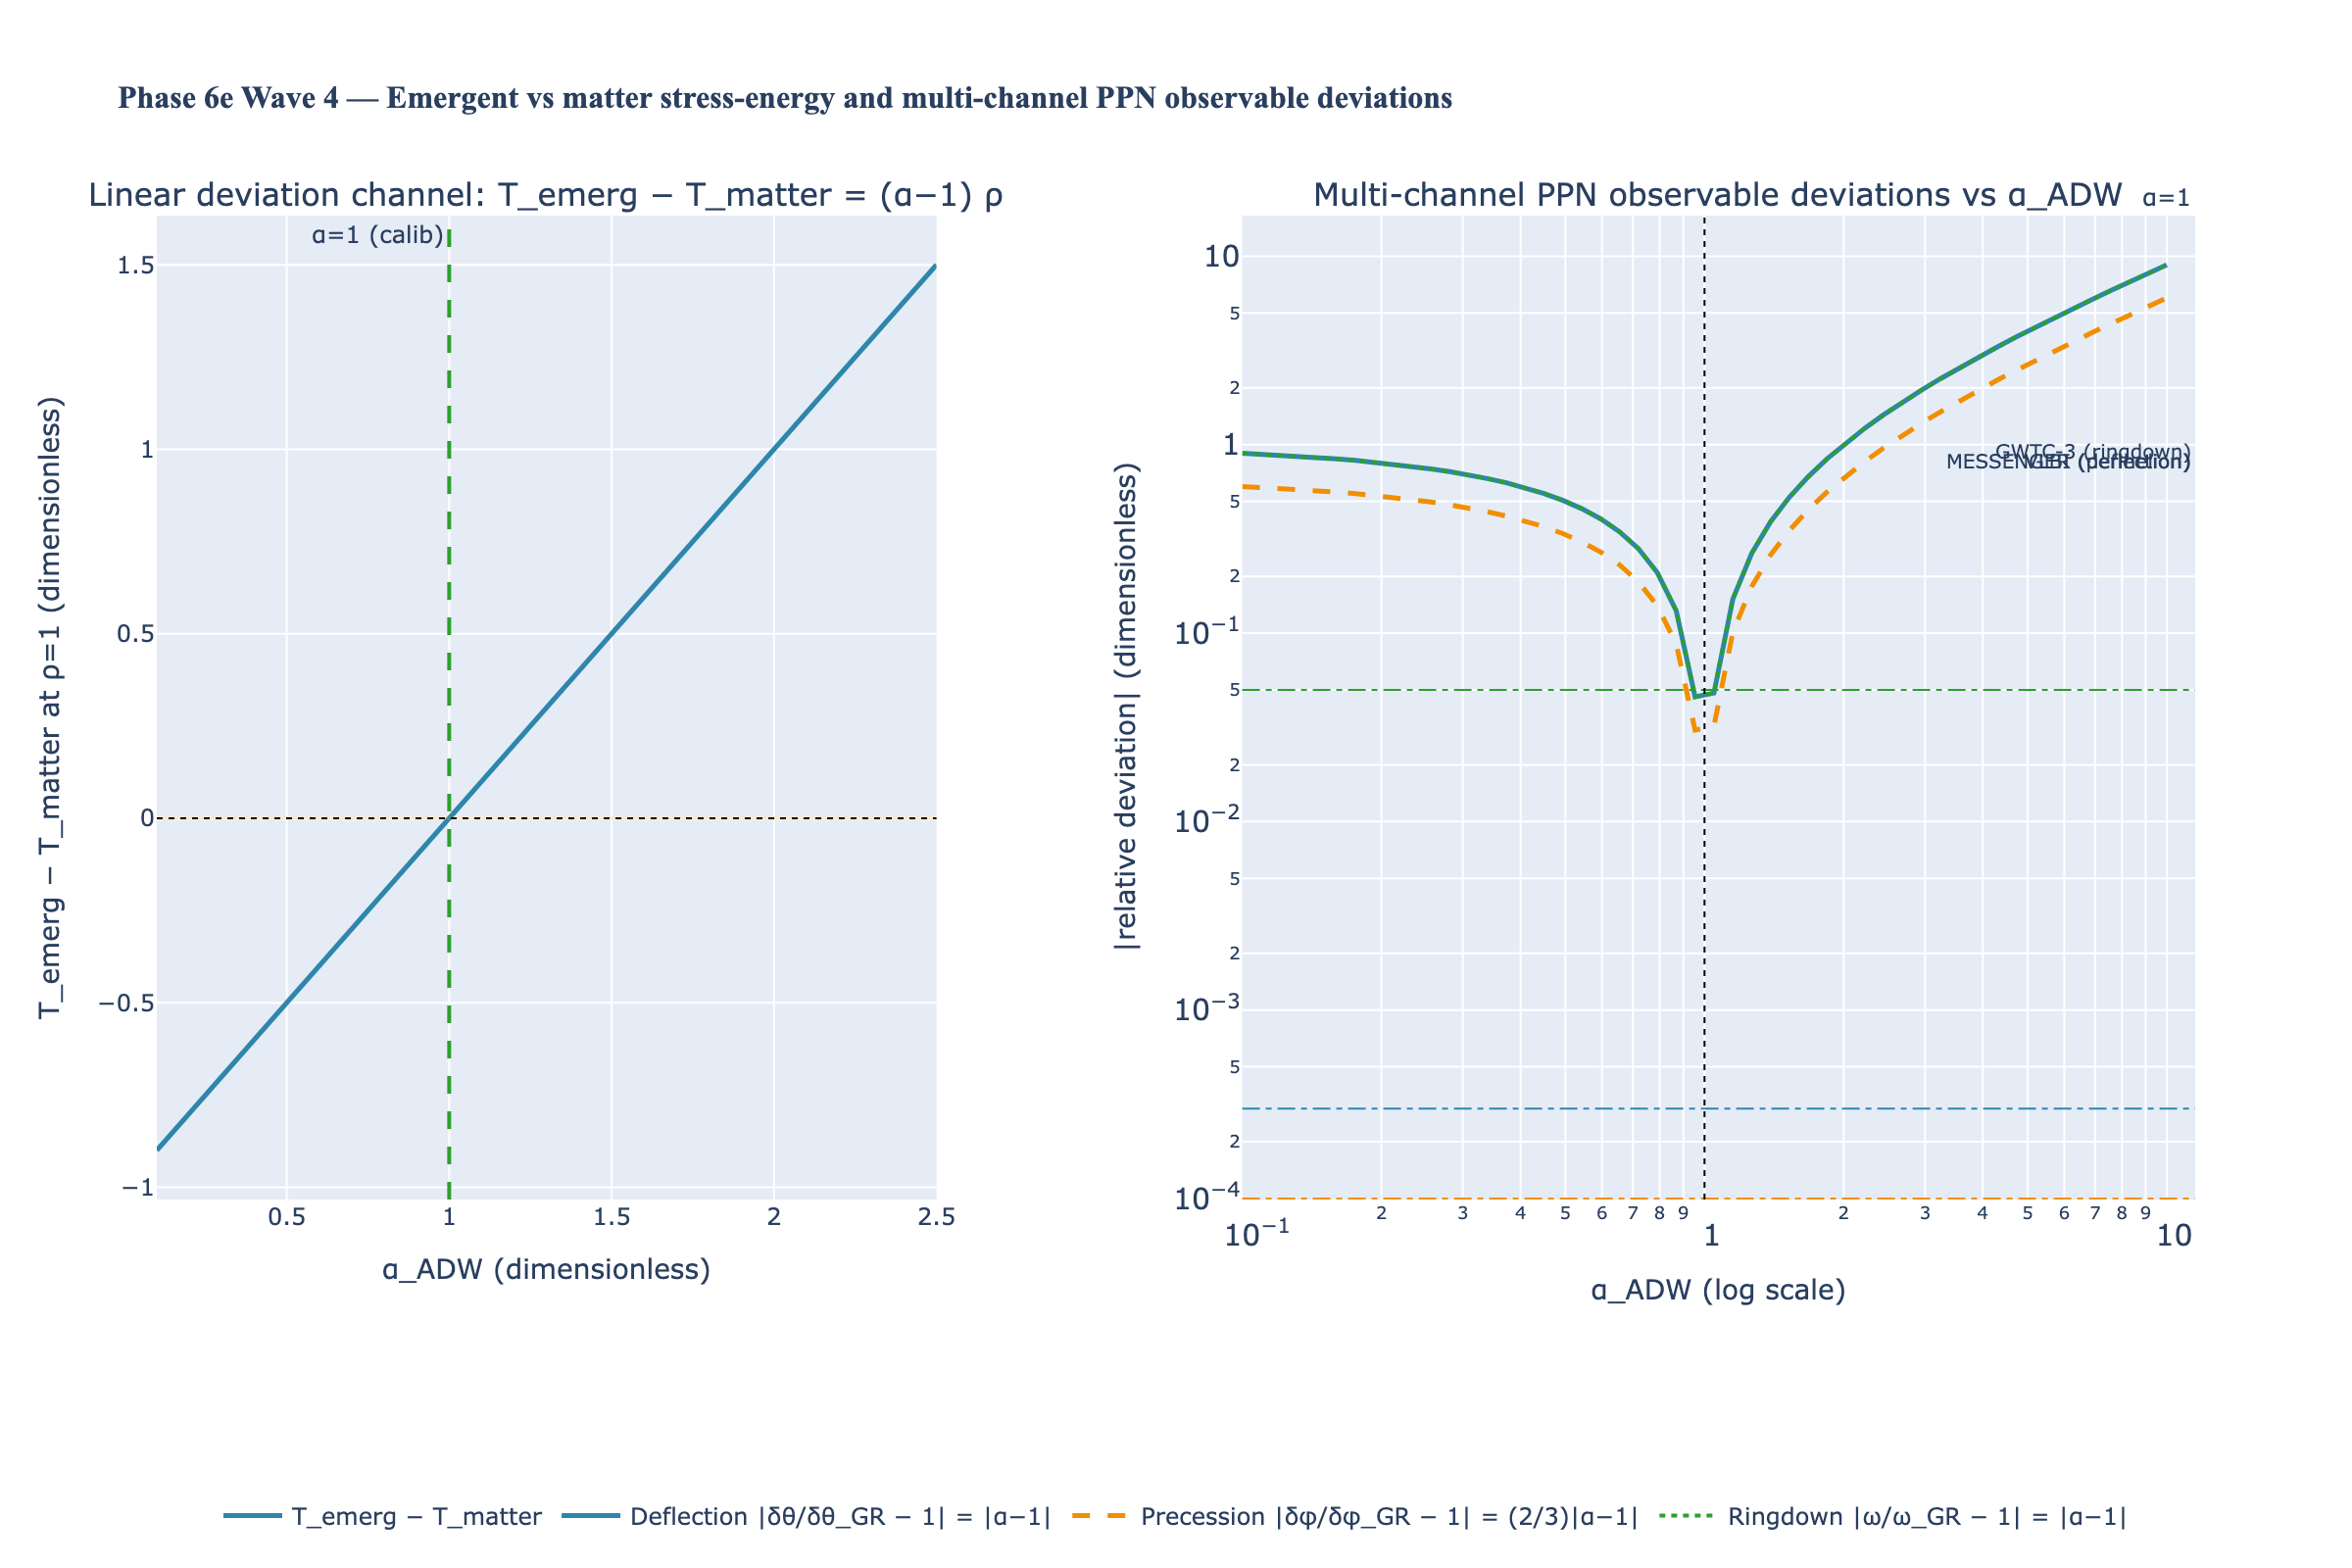
\includegraphics[width=0.95\linewidth]{figures/fig_T_emerg_vs_matter.png}
  \caption{Phase~6e Wave~4 --- emergent vs matter stress-energy and
    multi-channel PPN observable deviations under the ADW
    $\aADW$ rescaling. \emph{Left panel}: linear-in-$(\aADW - 1)$
    deviation channel $\Temerg - \Tmatter = (\aADW - 1) \cdot \rhoADW$
    at unit $\rhoADW$; vanishes at the Sakharov--Adler calibration
    $\aADW = 1$. The amber band marks the $5 \times 10^{-3}$ detection
    floor. \emph{Right panel}: log-log relative-deviation for three
    observables --- deflection ($|\aADW - 1|$), perihelion precession
    ($(2/3) |\aADW - 1|$), ringdown ($|\aADW - 1|$) --- over the
    natural Vergeles band $\aADW \in [0.1, 10]$. Cross-channel
    structural claim: $\delta\varphi/\delta\theta = 2/3$ at every
    $\aADW$ (Lean theorem
    \texttt{precession\_dev\_eq\_two\_thirds\_deflection\_dev}).
    Observation floors (VLBI $3 \times 10^{-4}$, MESSENGER
    $1 \times 10^{-4}$~\cite{Will2018}; GWTC-3 ringdown spectroscopy
    $5 \times 10^{-2}$~\cite{Berti2015}) drawn as dashed lines.}
  \label{fig:T_emerg_vs_matter}
\end{figure*}

\section{Substantive cross-bridges}
\label{sec:cross_bridges}

\subsection{Wave~2: higher-curvature pulsar bound}

The trace-level higher-curvature correction
$\mathcal{A}_{4}(R^{2}, R_{\mu\nu}^{2}, R_{\mu\nu\rho\sigma}^{2})$
inherits Wave~2's correctness-push pulsar
bound~\cite{HigherCurvature2026}: each Wave~1 Christensen--Duff
coefficient $|c_{R^{2}}|, |c_{R_{\mu\nu}^{2}}|, |c_{R_{\mu\nu\rho\sigma}^{2}}|
< 10^{59}$ at SM-relevant $\Nf \in [1, 100]$. Wave~4 closes this loop
into a trace-level statement: at any background curvature inputs,
\begin{equation*}
  |\mathcal{A}_{4}(\cdot, \cdot, \cdot)|
    \le \big(|R^{2}| + |R_{\mu\nu}^{2}| + |R_{\mu\nu\rho\sigma}^{2}|\big)
       \cdot 10^{59}.
\end{equation*}
The Lean proof (\texttt{higherCurvatureCorrection\_abs\_bound})
combines the Wave~2 main theorem with a triangle-inequality bound on
the three-channel sum.

\subsection{Wave~3: path-(b) diff invariance}

Wave~3's Decision Gate~E.3 verdict (PASS) certifies that the
variational EOM is well-posed at order $a_{4}$~\cite{DiffInvariance2026}.
Wave~4 consumes the bundled tracked-Prop
$H_{\mathrm{NonlinearDiffInvariance}}(diracCoefBundle\;\Nf, \Nf)$
directly through theorem \texttt{dirac\_H\_NonlinearDiffInvariance}
in Wave~3.

\section{Bundled tracked-Prop and Dirac witness}
\label{sec:bundle}

We bundle the substantive Wave~4 content into a single Prop:
\begin{equation}
  H_{\mathrm{NonlinearEFEHolds}}(\Lambda, \Nf, \rhoADW, \aADW) :\equiv
  \begin{cases}
    \mathcal{R}_{\mathrm{EFE}}(\GNem(\Lambda, \Nf, \aADW), \rhoADW, \aADW) = 0, \\
    H_{\mathrm{HigherCurvatureWithinObservationalBounds}}(10^{59}), \\
    H_{\mathrm{NonlinearDiffInvariance}}(diracCoefBundle\;\Nf, \Nf).
  \end{cases}
  \nonumber
\end{equation}
Each conjunct is a substantive cross-bridge consuming a different
Wave (Wave~4, Wave~2, Wave~3 respectively) by name; the bundle is
not P2 redundancy.

\begin{theorem}[Dirac calibration witness]\label{thm:bundle_witness}
For all $(\Lambda, \Nf, \rhoADW)$, the bundled Prop is satisfied at
the Sakharov--Adler calibration $\aADW = 1$:
\begin{equation*}
  H_{\mathrm{NonlinearEFEHolds}}(\Lambda, \Nf, \rhoADW, 1).
\end{equation*}
\end{theorem}
\noindent The Lean proof
(\texttt{dirac\_H\_NonlinearEFEHolds\_at\_alpha\_one}) discharges the
three conjuncts by direct invocation of
\texttt{efeResidualTrace\_at\_dirac\_calibration\_vanishes},
\texttt{H\_HigherCurvatureWithinObservationalBounds\_pulsar\_witness}
(Wave~2), and \texttt{dirac\_H\_NonlinearDiffInvariance} (Wave~3).

\begin{theorem}[Falsifier]\label{thm:bundle_falsifier}
Under positive $(\Lambda, \Nf)$, non-zero $\rhoADW$, positive $\aADW$,
and $\aADW \neq 1$, the bundled Prop is \emph{not} satisfied:
\begin{equation*}
  \neg\, H_{\mathrm{NonlinearEFEHolds}}(\Lambda, \Nf, \rhoADW, \aADW).
\end{equation*}
\end{theorem}
\noindent The Lean proof
(\texttt{perturbed\_alpha\_not\_H\_NonlinearEFEHolds}) extracts the
first conjunct, applies the Decision-Gate biconditional
$\mathcal{R}_{\mathrm{EFE}} = 0 \iff \aADW = 1$, and contradicts
$\aADW \neq 1$. The biconditional applicability requires
$\GN > 0$, which is supplied through the chain
$\aADW > 0 \Rightarrow \GNem(\Lambda, \Nf, \aADW) > 0$ via Phase~6a.1's
\texttt{LinearizedEFE.G\_N\_emerg\_pos} (consuming Vergeles
positivity~\cite{LinearizedEFE2026}). Substantive scope: this rules
out the trivial reading ``any $\aADW$ satisfies the bundle''; the
predicate \emph{genuinely} singles out the Sakharov--Adler calibration.

\section{Lean module structure}
\label{sec:lean_module}

The complete \texttt{NonlinearEFE.lean} module ships
\nonlinearEFEThms{} substantive theorems, zero \texttt{sorry}, and
zero new axioms. It is organised in six sections:

\begin{description}
  \item[\S1] \texttt{emergentStressEnergyTrace}, \texttt{matterStressEnergyTrace},
    \texttt{efeResidualTrace}, \texttt{higherCurvatureCorrection},
    \texttt{deflectionRatio}, \texttt{precessionRatio}, \texttt{ringdownRatio}
    (definitions only).
  \item[\S2] Stress-energy theorems: emergent--matter biconditional;
    linear deviation channel; positivity bridge (3 theorems).
  \item[\S3] EFE residual theorems: at-calibration vanishing; MAIN
    Decision-Gate biconditional; substantive Dirac calibration witness
    (3 theorems).
  \item[\S4] Observable signatures: deflection-deviation linearity;
    perihelion biconditional (non-trivial PPN combination);
    cross-channel $2/3$ ratio; quantitative VLBI floor falsifier
    (4 theorems).
  \item[\S5] Cross-bridges to Wave~2 (higher-curvature pulsar bound)
    (1 theorem).
  \item[\S6] Bundled tracked-Prop $H_{\mathrm{NonlinearEFEHolds}}$ +
    Dirac witness + perturbed-bundle falsifier (2 theorems).
\end{description}

The module imports \texttt{LinearizedEFE} (Phase~6a.1),
\texttt{HeatKernelExpansion} (Wave~1), \texttt{HigherCurvatureStructure}
(Wave~2), and \texttt{NonlinearDiffInvariance} (Wave~3) for its
substantive cross-bridges. Each cross-module reference in the
proof bodies is a \emph{named call} into the upstream Wave's main
result, providing P6 drift-protection per the project's
\texttt{feedback\_python\_lean\_refs\_drift.md} convention.

The Python mirror in \texttt{src/nonlinear\_efe/} provides numerical
evaluators for the trace-level residual, the multi-channel observable
signatures, and the bundled predicate; an
\nonlinearEFETests{}-case \texttt{pytest} suite cross-checks each
Lean theorem against the Wave~1, Wave~2, and Wave~3 numerics.

\section{Conclusion}
\label{sec:conclusion}

Phase~6e Wave~4 closes the variational nonlinear-EFE step in the ADW
emergent-gravity programme: at the trace level, the Decision-Gate
biconditional pins $\aADW = 1$ as the \emph{unique} ADW calibration
value at which the trace-level EFE closes, and PPN-style multi-channel
observables share an over-constrained $(\delta\theta, \delta\varphi,
\delta\omega) \propto \aADW - 1$ structure with the testable $3:2$
deflection-to-precession ratio. The bundled tracked-Prop
$H_{\mathrm{NonlinearEFEHolds}}$ consumes Wave~1 (heat-kernel
$\GN$), Wave~2 (higher-curvature pulsar bound), and Wave~3 (path-(b)
diff invariance) as load-bearing inputs, providing a single
substantive Lean handle for downstream Waves~5--6 (cosmological
constant, Einstein--Cartan extension).

\textsc{Forward look.} Wave~5 will extend the trace-level structure
to the microscopic-to-macroscopic coefficient match: expressing
$\GN^{\mathrm{emerg}}, \Lambda^{\mathrm{emerg}}$, and the
higher-curvature couplings in terms of $(\Lambda_{\mathrm{UV}}, \Nf,
G_{c})$ and testing the natural-parameter prediction against the
observed cosmological constant. Wave~6 will incorporate torsion
through the Einstein--Cartan extension. Both Waves consume the
bundled tracked-Prop $H_{\mathrm{NonlinearEFEHolds}}$ as a starting
input.

\begin{thebibliography}{99}

\bibitem{Wald1984}
R.~M.~Wald,
\emph{General Relativity},
University of Chicago Press, 1984;
ISBN 978-0-226-87033-5.

\bibitem{Will2018}
C.~M.~Will,
\emph{Theory and Experiment in Gravitational Physics} (2nd ed.),
Cambridge University Press, 2018;
DOI: 10.1017/9781316338612.

\bibitem{ChristensenDuff1979}
S.~M.~Christensen and M.~J.~Duff,
\emph{New gravitational index theorems and supertheorems},
Nucl. Phys. B \textbf{154}, 301 (1979).

\bibitem{Vassilevich2003}
D.~V.~Vassilevich,
\emph{Heat kernel expansion: user's manual},
Phys. Rep. \textbf{388}, 279 (2003)
[arXiv:hep-th/0306138].

\bibitem{Stelle1977}
K.~S.~Stelle,
\emph{Renormalization of higher-derivative quantum gravity},
Phys. Rev. D \textbf{16}, 953 (1977).

\bibitem{Sakharov1968}
A.~D.~Sakharov,
\emph{Vacuum quantum fluctuations in curved space and the theory of
gravitation},
Sov. Phys. Dokl. \textbf{12}, 1040 (1968).

\bibitem{BertiCardosoStarinets2009}
E.~Berti, V.~Cardoso, and A.~O.~Starinets,
\emph{Quasinormal modes of black holes and black branes},
Class. Quantum Grav. \textbf{26}, 163001 (2009)
[arXiv:0905.2975].

\bibitem{Berti2015}
E.~Berti et al.,
\emph{Testing general relativity with present and future astrophysical
observations},
Class. Quantum Grav. \textbf{32}, 243001 (2015)
[arXiv:1501.07274].

\bibitem{Roehm2026Wave1}
J.~G.~Roehm,
\emph{Formal heat-kernel calibration of induced Newton's constant from
the ADW Dirac substrate}
(in preparation, Phase 6e Wave 1).

\bibitem{HigherCurvature2026}
J.~G.~Roehm,
\emph{Higher-curvature structure from the Dirac heat kernel:
microscopic predictions and observational ceilings}
(in preparation, Phase 6e Wave 2).

\bibitem{DiffInvariance2026}
J.~G.~Roehm,
\emph{Path-(b) order-by-order diffeomorphism invariance of the
Seeley--DeWitt heat-kernel effective action}
(in preparation, Phase 6e Wave 3).

\bibitem{LinearizedEFE2026}
J.~G.~Roehm,
\emph{Linearized Einstein equations from ADW microscopic theory}
(in preparation, Phase 6a Wave 1).

\end{thebibliography}

\end{document}
